%图表序号清零
\setcounter{table}{0}
\setcounter{figure}{0}

\subsection{\hei\xiaosan\textbf{本文卷积网络结构}}
  \begin{figure}[H]
    \centering
    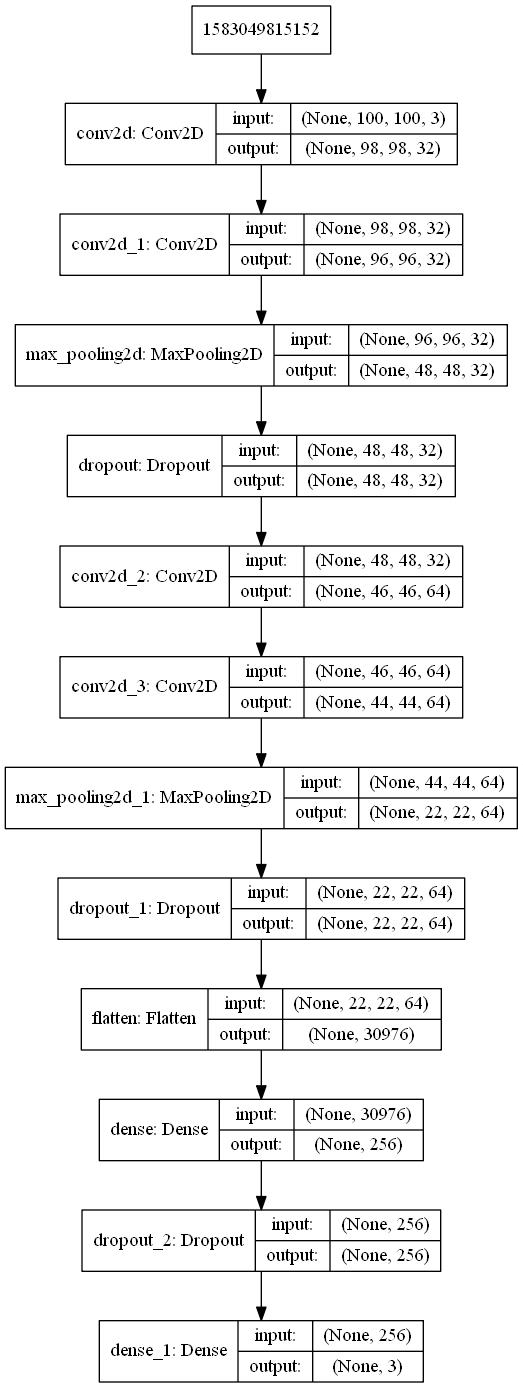
\includegraphics[width=.4\textwidth]{resource/NewbNet.png}
    \caption{本文网络结构}
    \label{Figure.Third.1}
  \end{figure}
  第一层和第二层为卷积层,它们的过滤器大小均为$3\times3$,深度为32,不使用全零填充,步长为1。
  第一层接受的输入\zerospace 层大小为$100\times100\times3$,所以输出的尺寸为$100+3-1=98$,深度为6。
  这一层共有$3\times3\times1\times32+32=320$个参数,其中32个为偏置。下一层节点矩阵有
  $98\times98\times32=307328$个节点,每个节点和$3\times3=9$个当前层节点相连,所以本卷积层
  共有$307328\times(9+1)=3073280$个连接。同理,第二层中共有$96\times96\times32\times(3\times3+1)=2949120$个连接。

  第三层为最大池化层,是一个$96\times96\times32$的节点矩阵。在本层中使用的过滤器大小为$2\times2$,步长为2.
  所以本层的输出大小为$48\times48\times16$。

  第四层为Dropout层,Dropout层是Hinton\cite{hinton2012improving}为了防止过拟合、提高
  神经网络的性能而提出的。该层会随机丢弃一些神经元,dropout rate为0.25。

  第五至八层结构与前四层相似,不过为了提取更深的特征,将深度增加为64层。

  第九层Flatten操作将输入$22\times22\times64$的张量展平为1维$1\times30976$的张量,
  为下一层的全连接操作做准备。

  第十层的全连接层(Dense)使用ReLU(RecitifiedLinearUnit,ReLU)作为激活函数。
  ReLU即线性整流函数,指代数学中的斜坡函数:$f(x)=max(0,x)$。
  该层输入大小为$30976$,输出节点个数为256个,总共参数为$30976\times256+256=7930112$个。

  第十一层仍为Dropout层,随机丢弃率为0.5。

  第十二层为全连接层,该层使用Softmax函数作为激活函数,该函数能将一个含任意实数的K维向量$\mathbf{Z}$
  “压缩”到另一个K维实向量$\sigma(\mathbf{Z})$中,并使得每一个元素的值域均在$(0,1)$之间,并且所有原色的和为1。
  该函数的形式通常由下式给出:
  \[
    \sigma(\mathbf{Z})_j=\frac{e^{z_j}}{\sum^\mathbf{K}_{k=1} e^{z_k}} \quad for\ j=1, \dots,\mathbf{K}
  \]
  该层输入大小为$256\times1$的张量,输出大小为3,即小麦病害类别个数。




\subsection{\hei\xiaosan\textbf{LeNet-5和AlexNet结构简介}}
  \begin{figure}[htbp]
    \centering
    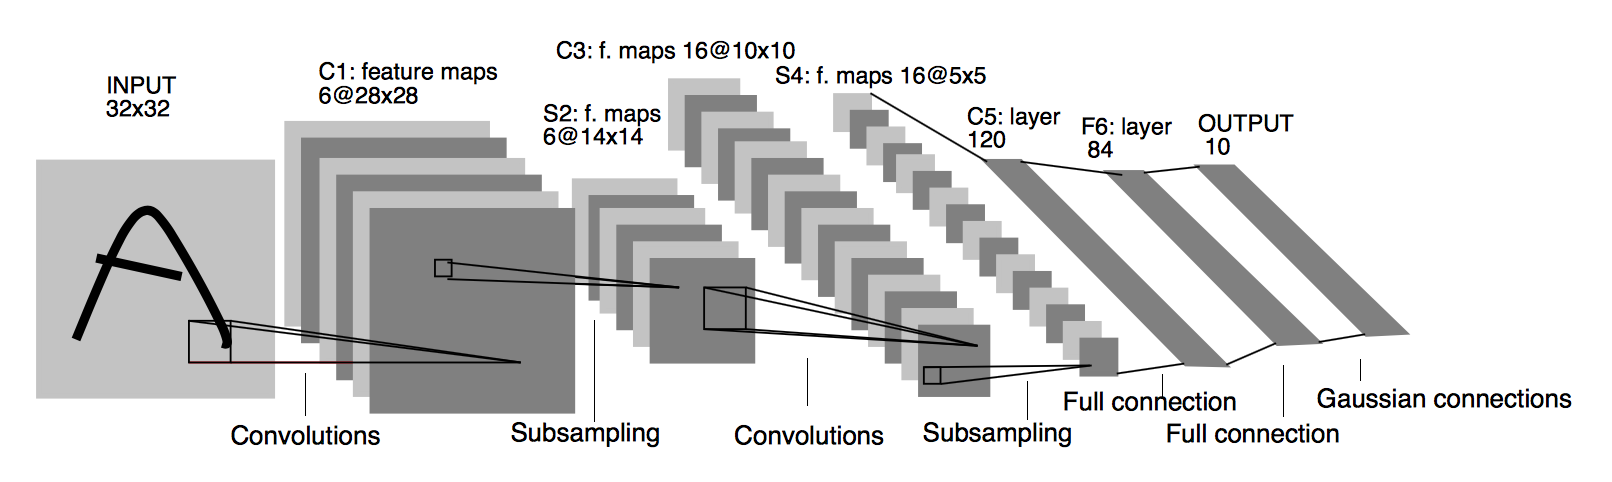
\includegraphics[width=\textwidth, natwidth=1612, natheight=482]{resource/2.4-网络结构.png}
    \caption{LeNet-5网络结构}
    \label{Figure.Third.2}
  \end{figure}
  第一层输入的是原始像素,LeNet-5模型接受的输入层\zerospace 大小为$32\times32\times1$。
  第一个卷积层过滤器\zerospace 尺寸为$5\times5$,深度为6,不使用全零填充,步长为1,
  输出尺寸为$32-5+1=28$,深度为6。这层共有$5\times5\times1\times6+6=156$个参数,其中6个为偏置。
  下一层的节点矩阵有$28\times28\times6=4704$个节点,每个节点和$5\times5=25$给节点相连,所以本层共有
  $4704\times(25+1)=122304$个连接。

  第二层池化层的输入\zerospace 是$28\times28\times6$的节点矩阵。该层的过滤器大小为$2\times2$,步长也为2。
  所以本层输出\zerospace 大小为$14\times14\times6$。第三层是输入大小为$14\times14\times6$的卷积层,卷积核大小为
  $2\times2$,步长为2。第四层是输入大小为$10\times10\times6$的卷积层,过滤器大小为$2\times2$,步长为2。
  第五至七层均为全连接层,最后一层的输出为10个预测值。


  \begin{figure}[htbp]
    \centering
    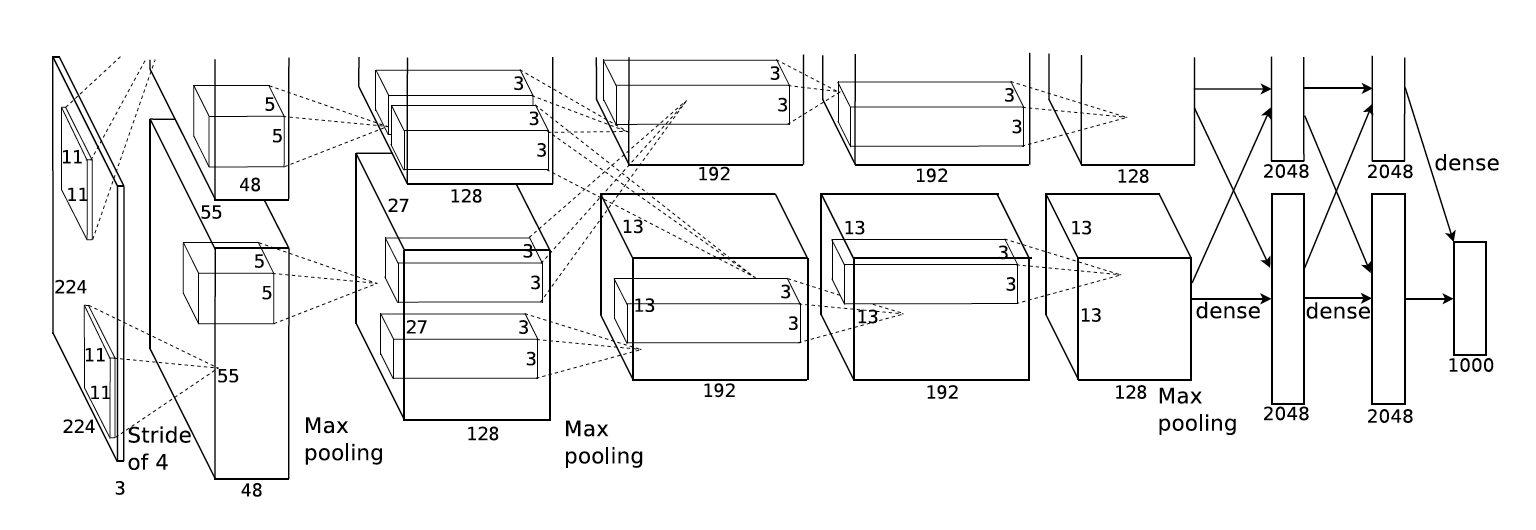
\includegraphics[width=\textwidth]{resource/AlexNet.png}
    \caption{AlexNet网络结构}
    \label{Figure.Third.3}
  \end{figure}
  AlexNet的输入图片大小为$224\times224\times3$,第一个卷积层使用96个较大的卷积核($11\times11$)
  步长为4;接着是LRN层;在之后是一个过滤器为$3\times3$的最大池化层,步长为2。接下来的卷积层中使用
  的卷积核都是$3\times3$或$5\times5$的大小,并且步长均为1。最大池化层依然是$3\times3$,步长为2。
  最后是三个相连的全连接层,最后输出1000个预测结果。

\subsection{\hei\xiaosan\textbf{实验步骤及操作}}
  \subsubsection{\hei\sihao\textbf{数据的获取及处理}}
    实验所用的图片均来自网络。首先利用Python爬虫分别在百度图片和谷歌图片上爬取小麦的白粉病、
    叶枯病、锈病图片,保存至本地文件夹并做好备份。手工去除不清晰、含水印等劣质图片后,使用Python
    脚本将原始图片切割为多份$300px\times300px$的图片。然后将这些图片按3:1:1的比例随机分为train、
    test、evaluate三个数据集,使用Python将全部图片的尺寸缩小为$100px\times100px$后转为numpy数组,
    最后将这些数组序列化为$*.npy$文件,这样的做法
    为重复实验省去了磁盘$IO$和图片处理操作的时间。数据集的样本和比例分布如图\ref{Figure.Third.4}所示:
    \begin{figure}[H]
      \centering
      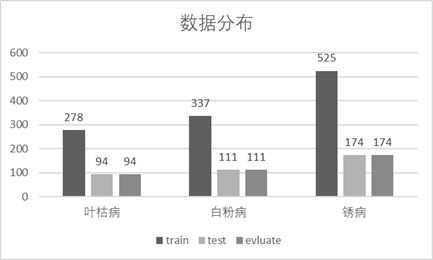
\includegraphics[width=.5\textwidth]{resource/数据分布.bmp}
      \caption{实验数据分布}
      \label{Figure.Third.4}
    \end{figure}

    \begin{figure}[htbp]
      \centering %图片全局居中
      \subfigure[叶枯病]{
        \begin{minipage}[t]{.2\textwidth}
          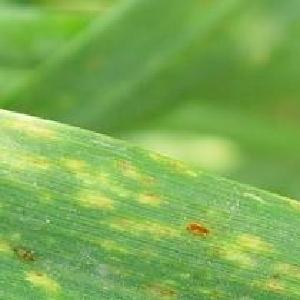
\includegraphics[width=\textwidth, natwidth=300, natheight=300]{resource/3.3叶枯病(1).jpg} \
          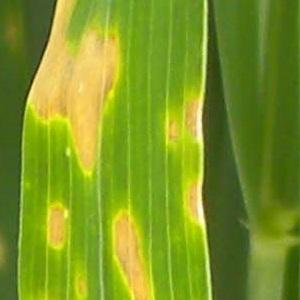
\includegraphics[width=\textwidth, natwidth=300, natheight=300]{resource/3.3叶枯病(2).jpg} \
          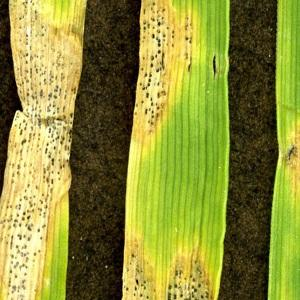
\includegraphics[width=\textwidth, natwidth=300, natheight=300]{resource/3.3叶枯病(3).jpg} \
        \end{minipage}
      }
      \subfigure[白粉病]{
        \begin{minipage}[t]{.2\textwidth}
          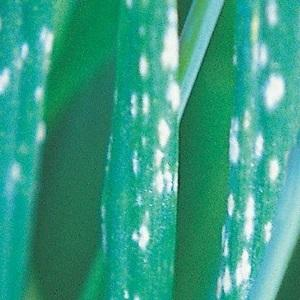
\includegraphics[width=\textwidth, natwidth=300, natheight=300]{resource/3.3白粉病(1).jpg} \
          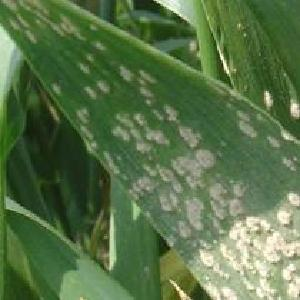
\includegraphics[width=\textwidth, natwidth=300, natheight=300]{resource/3.3白粉病(2).jpg} \
          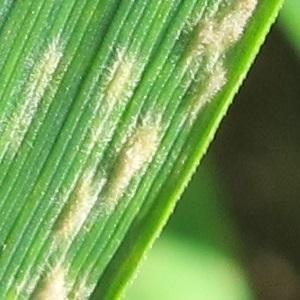
\includegraphics[width=\textwidth, natwidth=300, natheight=300]{resource/3.3白粉病(3).jpg} \
        \end{minipage}
      }
      \subfigure[锈病]{
        \begin{minipage}[t]{.2\textwidth}
          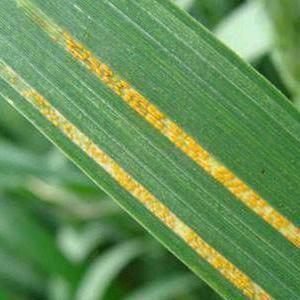
\includegraphics[width=\textwidth, natwidth=300, natheight=300]{resource/3.3锈病(1).jpg} \
          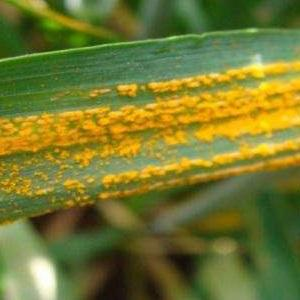
\includegraphics[width=\textwidth, natwidth=300, natheight=300]{resource/3.3锈病(2).jpg} \
          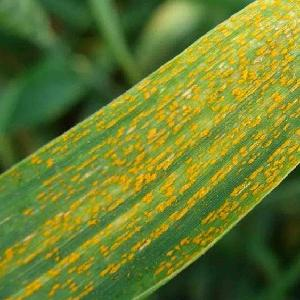
\includegraphics[width=\textwidth, natwidth=300, natheight=300]{resource/3.3锈病(3).jpg} \
        \end{minipage}
      }
      \caption{数据样本}
      \label{Figure.Third.5}
    \end{figure}
    % \begin{figure}
    %   \centering
    %   \subfigure[blight]{
    %     \begin{minipage}[t]{.2\textwidth}
    %       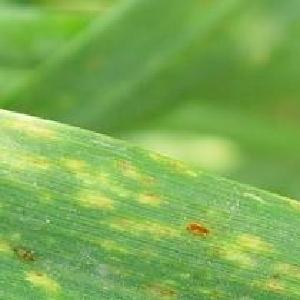
\includegraphics[width=\textwidth, natwidth=300, natheight=300]{resource/3.3叶枯病(1).jpg}
    %       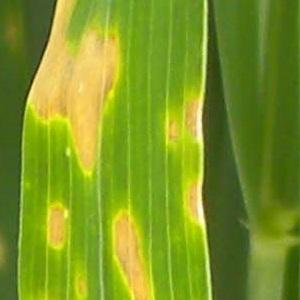
\includegraphics[width=\textwidth, natwidth=300, natheight=300]{resource/3.3叶枯病(2).jpg}
    %       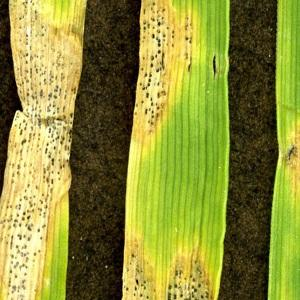
\includegraphics[width=\textwidth, natwidth=300, natheight=300]{resource/3.3叶枯病(3).jpg}
    %     \end{minipage}
    %   }
    %   \subfigure[powdery]{
    %     \begin{minipage}[t]{.2\textwidth}
    %       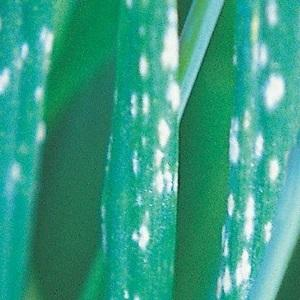
\includegraphics[width=\textwidth, natwidth=300, natheight=300]{resource/3.3白粉病(1).jpg}
    %       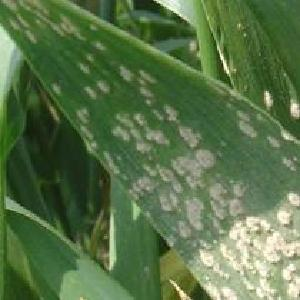
\includegraphics[width=\textwidth, natwidth=300, natheight=300]{resource/3.3白粉病(2).jpg}
    %       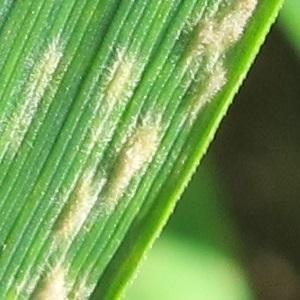
\includegraphics[width=\textwidth, natwidth=300, natheight=300]{resource/3.3白粉病(3).jpg}
    %     \end{minipage}
    %   }
    %   \subfigure[rust]{
    %     \begin{minipage}[t]{.2\textwidth}
    %       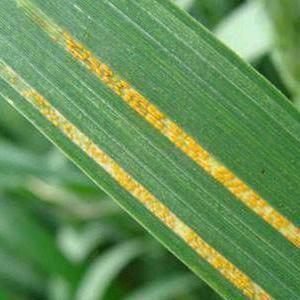
\includegraphics[width=\textwidth, natwidth=300, natheight=300]{resource/3.3锈病(1).jpg}
    %       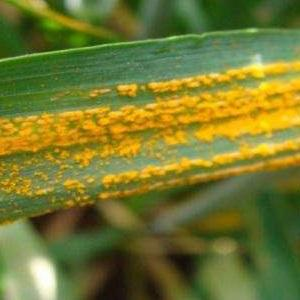
\includegraphics[width=\textwidth, natwidth=300, natheight=300]{resource/3.3锈病(2).jpg}
    %       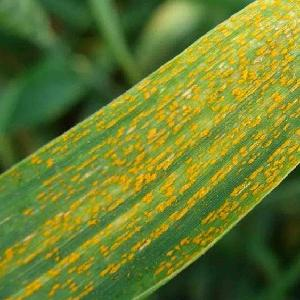
\includegraphics[width=\textwidth, natwidth=300, natheight=300]{resource/3.3锈病(3).jpg}
    %     \end{minipage}
    %   }
    % \end{figure}


  \subsubsection{\hei\sihao\textbf{卷积网络模型的建立}}
    在机器学习异常火热的今天,越来越多的机器学习库可供大家学习。本文使用最受欢迎的深度学习框架
    $TensorFlow$搭建卷积网络模型,具体环境为:

    {\hei\dawu
    \begin{itemize}
      \item 操作系统:Windows 10 x64 Version 1809
      \item 处理器:Intel(R) Core(TM) i7-6700HQ CPU @ 2.60GHz
      \item 显卡:Geforce GTX 950M
      \item 软件环境:
            \begin{itemize}
              \item Python 3.6.8 64-bit
              \item tensorflow-gpu 1.12.0
              \item keras 2.1.6-tf
              \item tensorboard 1.12.1
            \end{itemize}
    \end{itemize}
    }

    在TensorFlow中已经集成了Keras,它是使用Python编写的高级神经网络API,
    能够以TensorFlow作为后端运行。实验中为快速搭建卷积网络,使用Keras可节省大量时间。
    以下即为核心代码:

    \begin{lstlisting}
  model = Sequential()
  model.add(Conv2D(32, (3, 3), activation='relu', input_shape=(100, 100, 3)))
  model.add(Conv2D(32, (3, 3), activation='relu'))
  model.add(MaxPooling2D(pool_size=(2, 2)))
  model.add(Dropout(0.25))
  model.add(Conv2D(64, (3, 3), activation='relu'))
  model.add(Conv2D(64, (3, 3), activation='relu'))
  model.add(MaxPooling2D(pool_size=(2, 2)))
  model.add(Dropout(0.25))
  model.add(Flatten())
  model.add(Dense(256, activation='relu'))
  model.add(Dropout(0.5))
  model.add(Dense(3, activation='softmax'))
  sgd = SGD(lr=0.0001, decay=1e-6, momentum=0.01, nesterov=True)
  model.compile(loss='categorical_crossentropy', optimizer=sgd, metrics=['accuracy'])
    \end{lstlisting}

    为了便于实验后的数据分析,需要在代码中加入回调函数$keras.callbacks.TensorBoard$,
    设置了必要的参数后,程序在执行时便会在指定的文件夹写入运行过程的日志文件以供分析。
